\documentclass[times]{iapress}

\usepackage[colorlinks,bookmarksopen,bookmarksnumbered,citecolor=red,urlcolor=red]{hyperref}

\def\volumeyear{202x}
\def\volumenumber{x}
\def\volumemonth{Month}
\setcounter{page}{00}

\usepackage{amsmath,amssymb}
\usepackage{graphicx}
\usepackage{longtable,booktabs,array}
\usepackage[table]{xcolor}
\usepackage{newunicodechar}
\renewcommand{\baselinestretch}{1.01}

% ---- Unicode mappings so the manuscript compiles with pdfLaTeX ----
\newunicodechar{κ}{\ensuremath{\kappa}}
\newunicodechar{θ}{\ensuremath{\theta}}
\newunicodechar{φ}{\ensuremath{\varphi}}
\newunicodechar{ρ}{\ensuremath{\rho}}
\newunicodechar{β}{\ensuremath{\beta}}
\newunicodechar{γ}{\ensuremath{\gamma}}
\newunicodechar{η}{\ensuremath{\eta}}
\newunicodechar{α}{\ensuremath{\alpha}}
\newunicodechar{⌈}{\ensuremath{\lceil}}
\newunicodechar{⌉}{\ensuremath{\rceil}}
\newunicodechar{−}{\ensuremath{-}}
\newunicodechar{§}{\S}
\newunicodechar{¹}{\textsuperscript{1}}
\newunicodechar{³}{\textsuperscript{3}}
\newunicodechar{⁰}{\textsuperscript{0}}
\newunicodechar{⁻}{\textsuperscript{$-$}}
\newunicodechar{₀}{\textsubscript{0}}
\newunicodechar{Á}{\'A}
\newunicodechar{á}{\'a}
\newunicodechar{é}{\'e}
\newunicodechar{è}{\`e}
\newunicodechar{ì}{\`i}
\newunicodechar{č}{\v{c}}
\newunicodechar{ū}{\={u}}
\newunicodechar{ė}{\.{e}}

\begin{document}

\runningheads{Uncertainty-aware trade execution for VWAP-benchmarked order scheduling}{A. Irshad and S. Biswas}

\title{Uncertainty-Aware Trade Execution: Conformal Gating versus Reinforcement Learning for VWAP-Benchmarked Order Scheduling}

\author{Asadullah Irshad \affil{1}\corrauth,
   Shaon Biswas \affil{1}
 }

\address{
\affilnum{1}Centre of Excellence for Data Science, Artificial Intelligence and Modelling (DAIM), University of Hull, UK
}

\corraddr{Asadullah Irshad (Email: asadullahirshad3@gmail.com). Centre of Excellence for Data Science, Artificial Intelligence and Modelling (DAIM), University of Hull, UK.}

\begin{abstract}
Optimal trade execution, the problem of scheduling a large parent order over a trading session so as to minimise cost against a benchmark, is a sequential decision task that appears well suited to learning-based control. Yet a good deal of the reported progress fails to reproduce. We study the volume-weighted average price (VWAP) execution problem in a controlled and fully reproducible simulator with stochastic volatility and AR(1) return momentum. Within a single Markov decision process formulation, we compare classical schedules (TWAP, Almgren--Chriss, VWAP-tracking), a proximal-policy-optimisation (PPO) agent, and forecast-driven policies built on a normalised split-conformal predictor of next-interval returns. The predictor attains valid marginal coverage, 90.2\% empirical at a 90\% nominal level. Acting on its point forecast lowers mean slippage below VWAP-tracking but inflates cost variance. Gating those bets by the conformal interval half-width instead yields a tunable and monotone reduction of cost variability, from 19.1 to 10.0 bps, at negligible mean cost, tracing an explicit cost--risk frontier controlled by a single threshold. The PPO agent, evaluated over three training seeds, is high-variance and does not reliably dominate the simple schedules. In this controlled setting, a distribution-free conformal gate thus offers a more reproducible and interpretable route to uncertainty-aware execution than an off-the-shelf reinforcement-learning agent. All code and the simulator are released. On real intraday data (thirty US large-caps, 5-minute bars) the predictor's coverage transfers closely (90.7\% empirical at the 90\% level) and the variance-reduction effect of gating persists, although the forecast edge itself is small, since real high-frequency returns are only weakly predictable.
\end{abstract}

\keywords{optimal execution; VWAP; conformal prediction; uncertainty quantification; reinforcement learning; Markov decision process; market microstructure.}

\maketitle

\noindent\footnotesize\emph{Both authors completed the MSc (Distinction) in Artificial Intelligence and Data Science at the University of Hull, affiliated with the DAIM Centre of Excellence. This study was conducted independently and did not receive funding or resources from the Centre.}\normalsize
\vskip 8pt%
\noindent{\bf AMS 2010 subject classifications} 91G80, 68T05
\vskip 8pt%
\noindent{\bf DOI:} 10.19139/soic-2310-5070-????

\section{Introduction}

For an institutional desk, the question is rarely whether to trade. The
position has usually been decided already, and what remains is an
operational problem: how to trade it. Pushed into the market too
quickly, an order moves the price against itself through market impact.
Worked too slowly, it is left exposed to adverse price drift over the
execution horizon. Algorithmic execution lives between these two costs,
and the volume-weighted average price (VWAP) is among the most common
benchmarks against which the quality of that trade-off is judged.

Since execution is a sequential decision made under uncertainty, it is a
natural candidate for reinforcement learning (RL), and a large body of
work now applies deep RL to trading and execution (Nevmyvaka et al.,
2006; Lin \& Beling, 2020; Ning et al., 2021; Hambly et al., 2023; Macrì
\& Lillo, 2024). A recurring criticism, however, is that the reported
gains are hard to reproduce. Experimental settings differ from paper to
paper, market-impact assumptions are often left unstated, and
conclusions frequently rest on a single training run. We take the
opposite stance here and ask a narrower question: which approaches
deliver cost reductions that are robust, controllable, and reproducible,
the properties an execution desk actually cares about?

This paper makes three contributions. First, we release a compact,
self-contained execution simulator with stochastic volatility and AR(1)
momentum, in which short-horizon returns are partially predictable but
carry time-varying uncertainty. Second, we construct a normalised
split-conformal predictor of next-interval returns whose
distribution-free interval width tracks local volatility, and we use
that interval to gate forecast-driven trading. Third, we place classical
schedules, a multi-seed PPO agent, and the conformal policies on a
common cost--risk frontier for a like-for-like comparison. The central
finding is that the conformal gate converts an unstable forecast edge
into a tunable variance reduction, and does so more reliably than the
learned agent.

\section{Related Work}

Classical execution theory treats the problem as a trade-off between
impact and risk. The Almgren--Chriss framework derives a deterministic
trajectory that is optimal under a mean--variance objective with linear
impact (Almgren \& Chriss, 2001) and remains the standard academic
baseline; it builds on the earlier optimal-control formulation of
execution cost of Bertsimas \& Lo (1998). Later work refined how impact
and its resilience are modelled (Obizhaeva \& Wang, 2013; Gatheral,
2010), while VWAP- and TWAP-tracking became the dominant practitioner
heuristics (Cartea et al., 2015). On the learning side, RL for execution
spans value-based, actor--critic, and risk-sensitive variants (Nevmyvaka
et al., 2006; Lin \& Beling, 2020; Ning et al., 2021; Nagy et al., 2023;
Macrì \& Lillo, 2024), and recent surveys document the rapid growth of
the area alongside persistent concerns about inconsistent evaluation and
overly optimistic frictions (Sun et al., 2023; Hambly et al., 2023;
Cartea et al., 2023). Conformal prediction, for its part, provides
distribution-free, finite-sample coverage for an arbitrary predictor
(Vovk et al., 2005; Lei et al., 2018; Angelopoulos \& Bates, 2023) and
has since been extended to quantile regression (Romano et al., 2019), to
time series (Stankevičiūtė et al., 2021; Xu \& Xie, 2023), and to
distribution shift (Tibshirani et al., 2019; Zaffran et al., 2022;
Barber et al., 2023; Gibbs \& Candès, 2024). Its use as an explicit gate
on execution decisions, however, has received little attention. We
connect these threads by using conformal intervals not to forecast
direction for alpha, but to decide when a short-horizon timing signal is
reliable enough to act on.

\section{Methodology}

Figure 1 summarises the method. At each interval, the market state feeds
a gradient-boosted return predictor; a normalised split-conformal layer
turns the resulting point forecast into a distribution-free interval;
and a gate compares the forecast against the width of its own interval,
then either acts on the signal or defers to the VWAP schedule. We detail
each component below.

\begin{figure}[htbp]
\centering
\begin{center}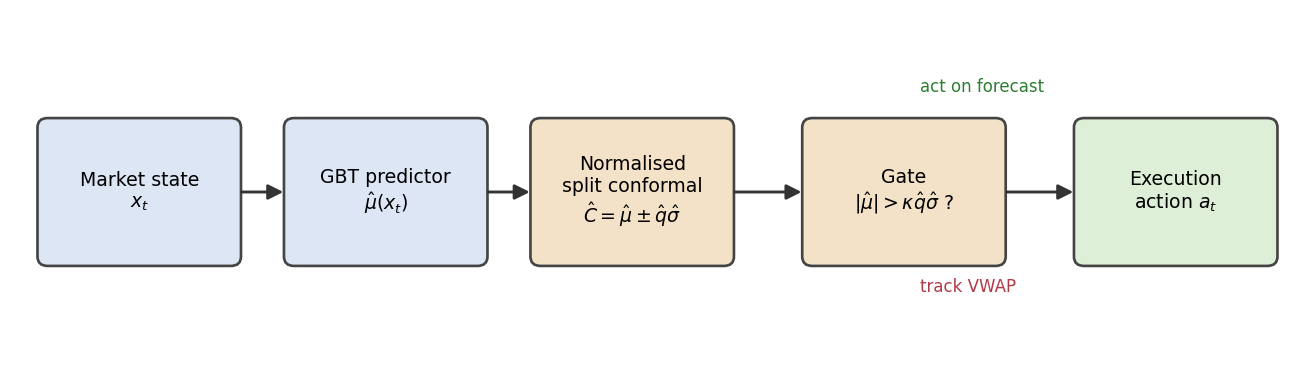
\includegraphics[width=4.600in,keepaspectratio]{./media/image1.png}\end{center}
\caption{The uncertainty-aware execution pipeline: a return predictor feeds a normalised split-conformal interval, whose width gates whether the policy acts on the forecast or tracks VWAP.}
\label{fig:1}
\end{figure}

\subsection{Market simulator}

Each episode is one trading session discretised into T intervals. The
log-return carries an AR(1) momentum term and is driven by a
stochastic-volatility process; the per-interval volatility follows a
log-AR(1) path inducing volatility clustering:

\begin{center}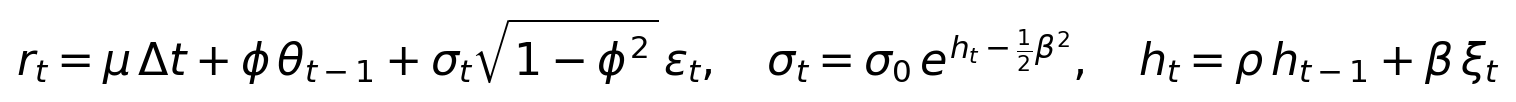
\includegraphics[width=4.600in,keepaspectratio]{./media/image2.png}\end{center}
where θ is the latent momentum state, h the log-volatility, and φ, ρ, β
control momentum persistence, volatility persistence, and vol-of-vol
respectively. Volume follows a U-shaped intraday profile with
multiplicative noise, and the benchmark is the volume-weighted mean
price:

\begin{center}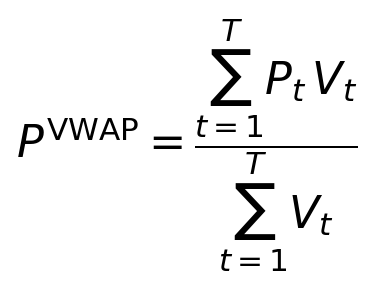
\includegraphics[width=2.500in,keepaspectratio]{./media/image3.png}\end{center}
A representative session is shown in Figure 2. The conformal forecast
band widens during volatile stretches and narrows in calm ones, so the
width of the band is itself an informative signal rather than a fixed
margin.

\begin{figure}[htbp]
\centering
\begin{center}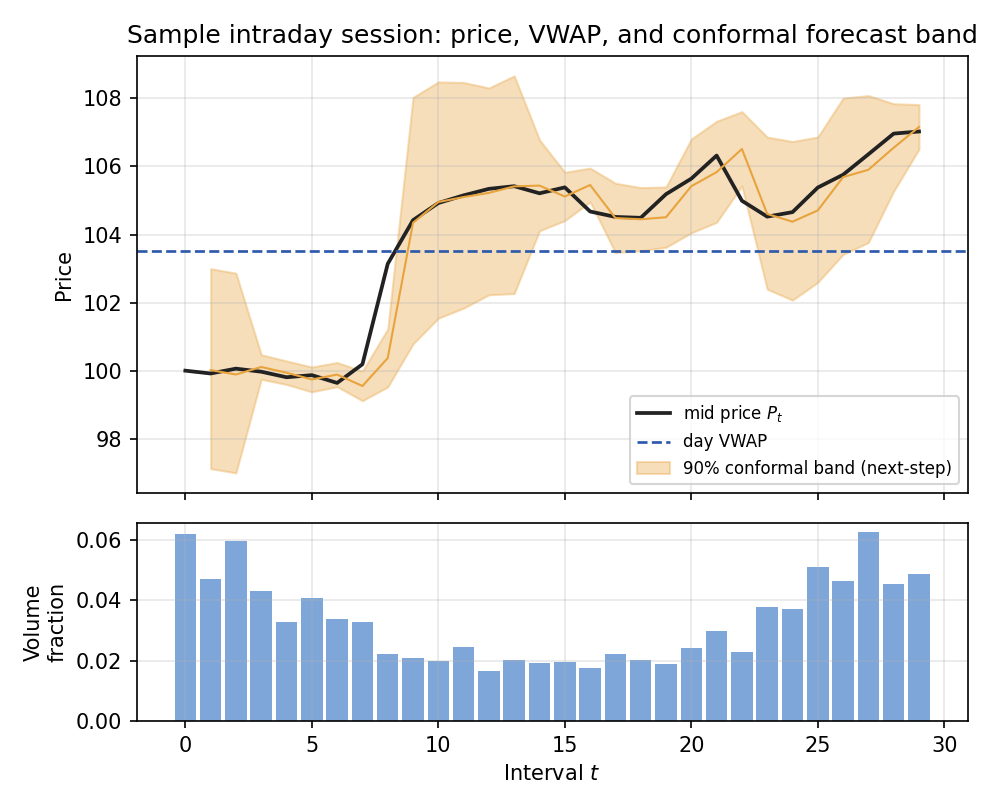
\includegraphics[width=4.479in,keepaspectratio]{./media/image4.png}\end{center}
\caption{A sample intraday session. Top: mid price, day VWAP, and the 90\% next-step conformal band, which widens in volatile periods. Bottom: the U-shaped market-volume profile.}
\label{fig:2}
\end{figure}

\subsection{Execution as a Markov decision
process}

The agent sells a parent order of Q shares over T intervals. We model
this as a Markov decision process (S, A, P, r, γ) (Sutton \& Barto,
2018). The state comprises the fraction of time and inventory remaining,
recent return, relative interval volume, and price relative to arrival
(with two optional conformal features, §3.5). The action is a
log-multiplier on the VWAP-tracking quantity, so a value of zero
reproduces volume-curve tracking; the executed quantity,
participation-rate impact, and realised price are

\begin{center}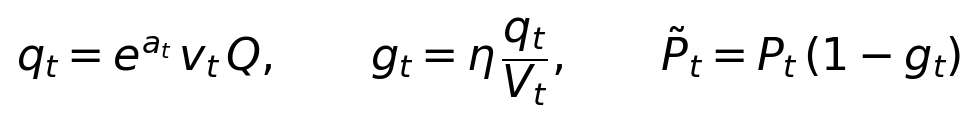
\includegraphics[width=4.583in,keepaspectratio]{./media/image5.png}\end{center}
Here v is the volume fraction, V the interval market volume, and η the
impact coefficient; the temporary impact is linear in the participation
rate (Figure 3). Writing the per-trade implementation shortfall (Perold,
1988) against the arrival price P₀ as

\begin{center}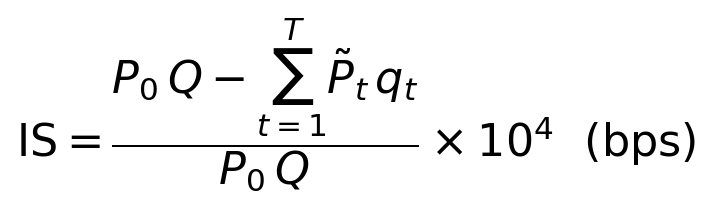
\includegraphics[width=3.958in,keepaspectratio]{./media/image6.png}\end{center}
the execution problem is the constrained stochastic optimisation

\begin{center}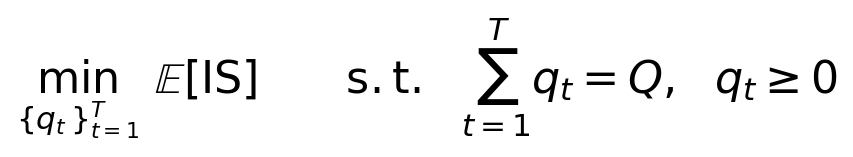
\includegraphics[width=3.958in,keepaspectratio]{./media/image7.png}\end{center}
\begin{figure}[htbp]
\centering
\begin{center}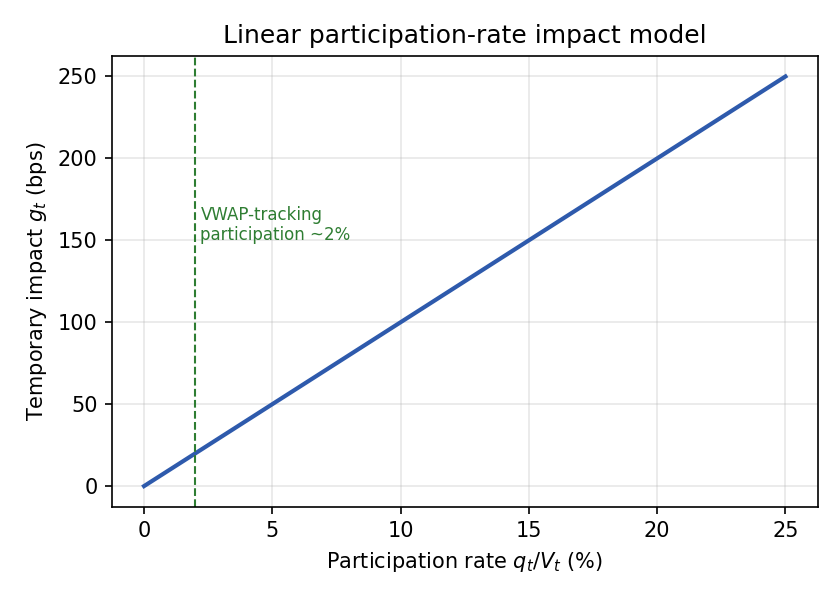
\includegraphics[width=3.750in,keepaspectratio]{./media/image8.png}\end{center}
\caption{Temporary impact as a function of participation rate (η = 0.1). Trading a larger share of an interval's volume is more expensive; VWAP-tracking holds participation low.}
\label{fig:3}
\end{figure}

The reward combines the per-interval implementation-shortfall
contribution (in basis points of the parent notional) with a
volatility-scaled penalty on deviations from the VWAP schedule,
representing the timing risk of a discretionary bet:

\begin{center}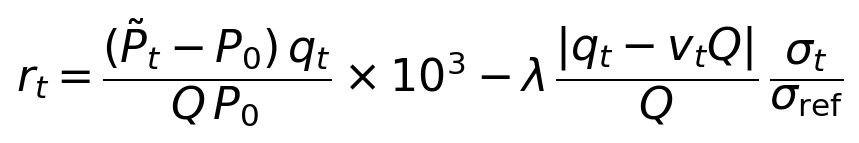
\includegraphics[width=4.600in,keepaspectratio]{./media/image9.png}\end{center}
\subsection{Classical baselines}

Immediate liquidates at the open. TWAP executes equal slices.
VWAP-tracking trades proportional to the volume curve. Almgren--Chriss
minimises a mean--variance execution cost (Almgren \& Chriss, 2001),

\begin{center}
\includegraphics[width=3.750in,keepaspectratio]{./media/image10.png}\end{center}
whose solution is the risk-averse closed-form trajectory

\begin{center}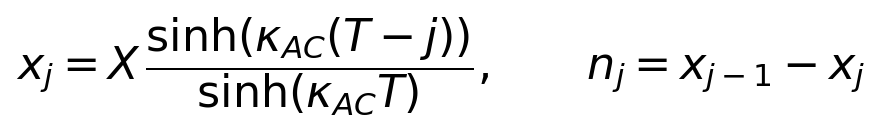
\includegraphics[width=3.958in,keepaspectratio]{./media/image11.png}\end{center}
where the urgency parameter sets the degree of front-loading. We map
each schedule into the common action parametrisation for an identical
evaluation pipeline.

\subsection{Normalised split-conformal
predictor}

We fit a gradient-boosted regressor that predicts the next-interval
return from causal features: recent returns, a rolling volatility
estimate, and time of day. Following the split-conformal construction of
Lei et al. (2018), with a local normalisation in the spirit of
conformalized quantile regression (Romano et al., 2019), we form
normalised nonconformity scores on a held-out calibration set (Figure
4), take the conformal quantile, and obtain a prediction interval whose
width scales with local volatility:

\begin{center}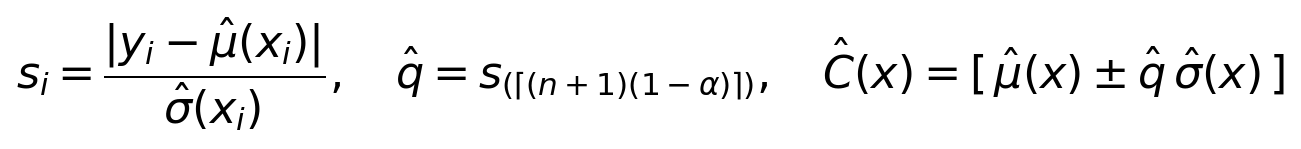
\includegraphics[width=4.600in,keepaspectratio]{./media/image12.png}\end{center}
\begin{figure}[htbp]
\centering
\begin{center}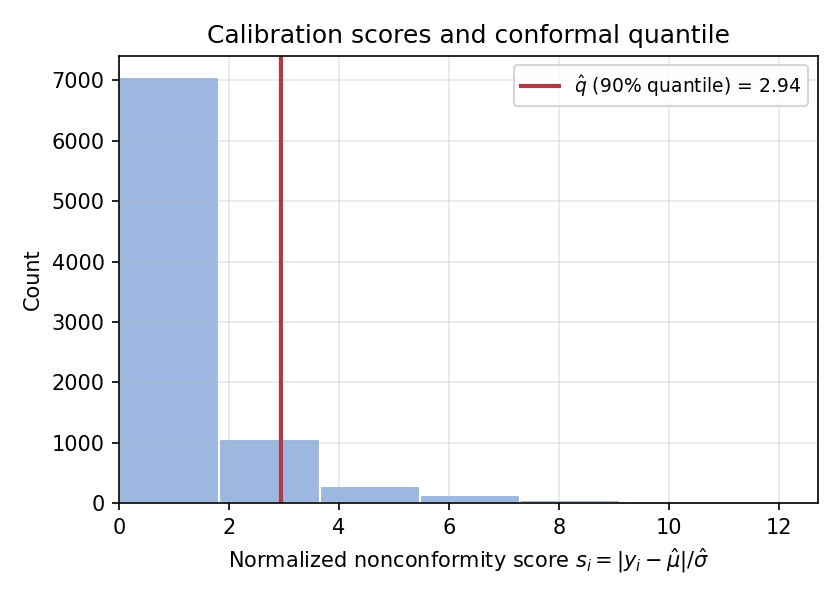
\includegraphics[width=3.750in,keepaspectratio]{./media/image13.png}\end{center}
\caption{Distribution of normalised nonconformity scores on the calibration set; the 90\% empirical quantile defines the conformal interval half-width.}
\label{fig:4}
\end{figure}

Under exchangeability this construction satisfies the standard
finite-sample coverage guarantee (Vovk et al., 2005; Lei et al., 2018),
stated below.

\textbf{Theorem 1 (marginal coverage).} \emph{If the calibration scores
and the test score are exchangeable, the prediction set satisfies}

\begin{center}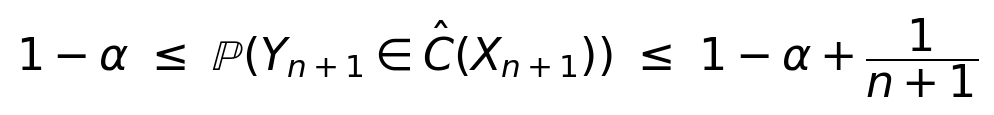
\includegraphics[width=4.479in,keepaspectratio]{./media/image14.png}\end{center}
Proof sketch. Under exchangeability, the rank of the test score among
the n calibration scores is uniform on \{1, \ldots, n+1\}. Taking the
conformal quantile as the ⌈(n+1)(1−α)⌉-th order statistic gives the
lower bound, and the upper bound follows from the discreteness of the
empirical quantile (Lei et al., 2018). Financial series, of course,
violate exchangeability. We mitigate this with the local-volatility
normalisation and verify coverage empirically (§5); online and
non-exchangeable conformal variants (Gibbs \& Candès, 2024; Zaffran et
al., 2022; Xu \& Xie, 2023; Barber et al., 2023) offer stronger
guarantees under drift, and we return to them in the limitations.

Figure 5 reports empirical coverage against the nominal level on fresh
simulated days. The curve tracks the diagonal closely, and at the
operating point alpha = 0.1 the empirical coverage is 90.2\%, confirming
validity out of sample.

\begin{figure}[htbp]
\centering
\begin{center}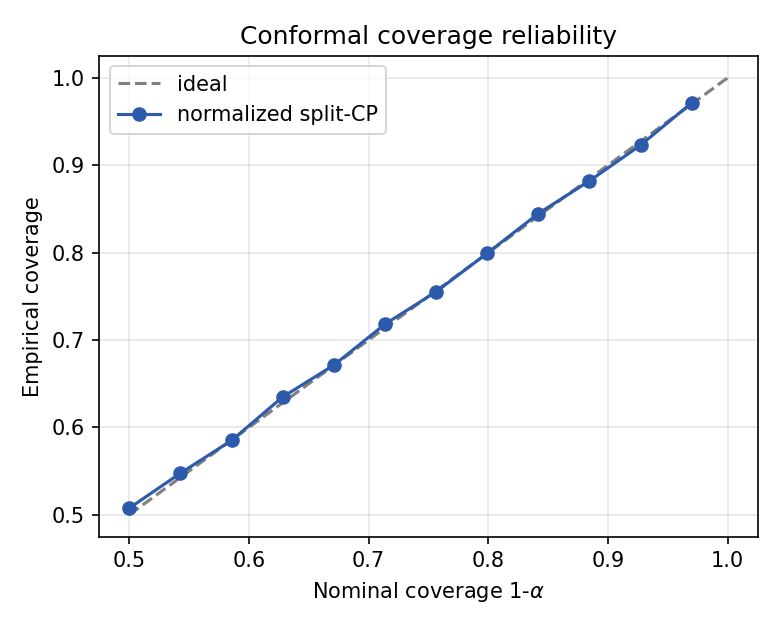
\includegraphics[width=3.750in,keepaspectratio]{./media/image15.png}\end{center}
\caption{Conformal coverage reliability. Empirical coverage of the normalised split-conformal interval against the nominal level on held-out simulated days; closeness to the diagonal indicates calibration.}
\label{fig:5}
\end{figure}

\subsection{Forecast-driven and gated
policies}

Two policies make use of the predictor. Forecast-greedy tilts the
schedule in the direction of the point forecast, irrespective of its
uncertainty. Conformal-gated tilts only when the absolute forecast
exceeds a multiple of the conformal half-width, that is, only when the
signal escapes its own uncertainty band; otherwise it tracks VWAP:

\begin{center}
\includegraphics[width=4.600in,keepaspectratio]{./media/image16.png}\end{center}
The threshold acts as a single interpretable dial. A value of zero
recovers Forecast-greedy, and large values recover VWAP-tracking. As
Figure 6 shows, the fraction of intervals in which the gate fires falls
as the threshold rises, making the policy progressively more
conservative.

\begin{figure}[htbp]
\centering
\begin{center}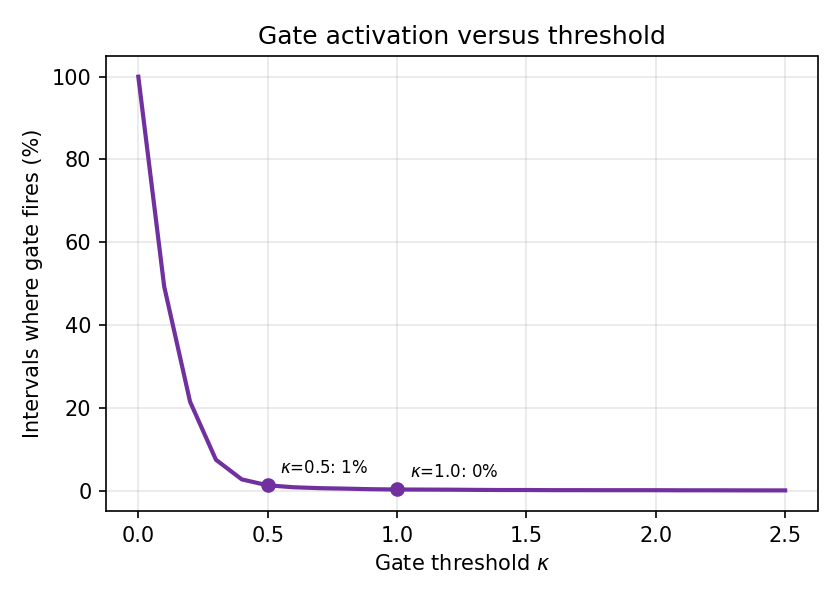
\includegraphics[width=3.750in,keepaspectratio]{./media/image17.png}\end{center}
\caption{Gate activation versus threshold: the fraction of intervals in which the forecast escapes its conformal band, and the policy acts, decreases monotonically with κ.}
\label{fig:6}
\end{figure}

\section{Experimental Setup}

All policies are evaluated on 250 held-out market seeds, disjoint from
any training or calibration data. The PPO agent (Schulman et al., 2017)
uses a two-layer network with normalised observations and rewards, is
trained for 150,000 timesteps, and is trained independently with three
seeds so that training-seed variability is exposed rather than hidden;
its statistics pool every evaluation episode across the three agents.
The headline metric is slippage versus VWAP, the gap between the
achieved average execution price and the day's VWAP, expressed in basis
points:

\begin{center}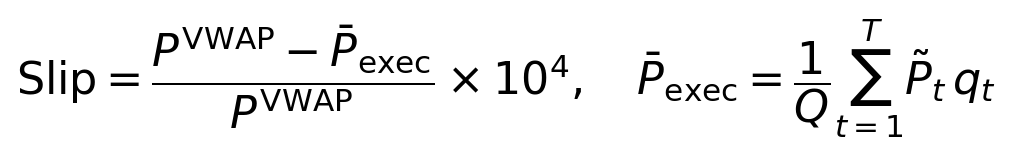
\includegraphics[width=4.600in,keepaspectratio]{./media/image18.png}\end{center}
We report the Monte-Carlo mean and standard deviation of this quantity
across the 250 episodes, which we read as cost and risk respectively,
with 95\% confidence intervals from a non-parametric bootstrap (2,000
resamples). Implementation shortfall against arrival is recorded as
well. The conformal nominal level is fixed at 90\% (alpha = 0.1).

\section{Results}

Table 1 summarises execution performance and Figure 7 plots each method
on the cost--risk plane.

\textbf{Table 1.} Execution performance over 250 held-out seeds. Lower
is better on both axes; conformal-gated rows highlighted.

\begin{longtable}[]{@{}llll@{}}
\toprule
\begin{minipage}[b]{0.22\columnwidth}\raggedright
\textbf{Method}\strut
\end{minipage} & \begin{minipage}[b]{0.22\columnwidth}\raggedright
\textbf{Slippage vs VWAP}

\textbf{mean (bps)}\strut
\end{minipage} & \begin{minipage}[b]{0.22\columnwidth}\raggedright
\textbf{Slippage vs VWAP}

\textbf{std (bps)}\strut
\end{minipage} & \begin{minipage}[b]{0.22\columnwidth}\raggedright
\textbf{Class}\strut
\end{minipage}\tabularnewline
\midrule
\endhead
Immediate & 332.1 & 296.8 & Naive\tabularnewline
TWAP & 25.1 & 38.0 & Schedule\tabularnewline
Almgren--Chriss & 50.8 & 237.3 & Schedule\tabularnewline
VWAP-tracking & 20.0 & 0.0 & Schedule\tabularnewline
PPO (RL, 3 seeds) & 33.9 & 115.9 & Learned\tabularnewline
Forecast-greedy & 17.0 & 19.1 & Forecast\tabularnewline
\rowcolor{gray!18}Conformal-gated ($\kappa$=0.5) & 19.1 & 13.8 & Conformal\tabularnewline
\rowcolor{gray!18}Conformal-gated ($\kappa$=1.0) & 19.4 & 10.0 & Conformal\tabularnewline
\bottomrule
\end{longtable}

\begin{figure}[htbp]
\centering
\begin{center}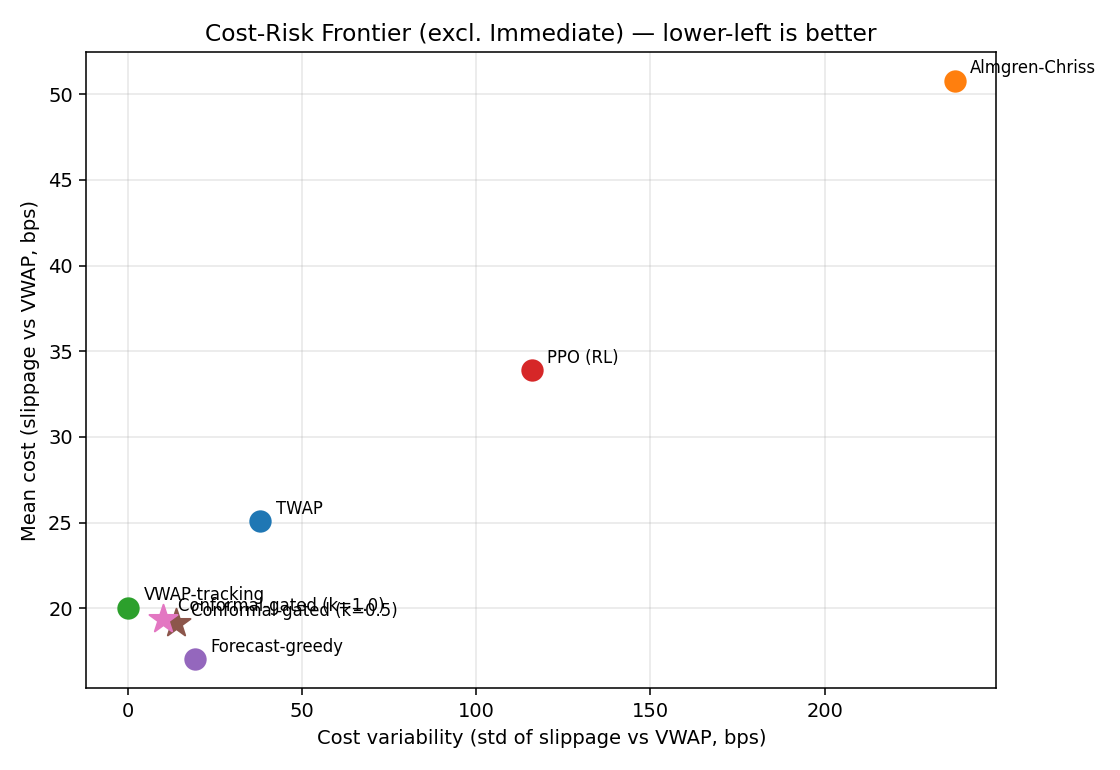
\includegraphics[width=4.600in,keepaspectratio]{./media/image19.png}\end{center}
\caption{Cost--risk frontier (Immediate omitted for scale). Lower-left is better; conformal-gated policies (stars) sit at low variance with near-best mean cost.}
\label{fig:7}
\end{figure}

Figure 8 reports the mean execution cost of each method with 95\%
bootstrap confidence intervals (2,000 resamples), which confirm that the
ordering of mean costs is not an artefact of sampling.

\begin{figure}[htbp]
\centering
\begin{center}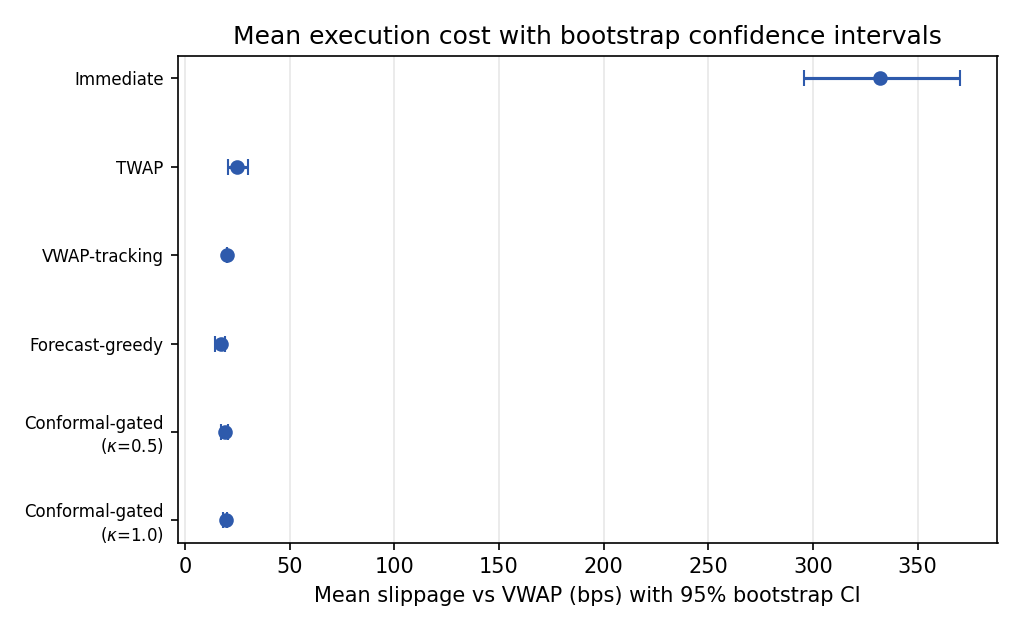
\includegraphics[width=4.375in,keepaspectratio]{./media/image20.png}\end{center}
\caption{Mean slippage versus VWAP with 95\% bootstrap confidence intervals over 250 held-out seeds.}
\label{fig:8}
\end{figure}

Three patterns stand out. First, VWAP-tracking is a strong reference
with essentially zero variance at 20.0 bps, because its only systematic
cost is impact, and the volume-proportional schedule is precisely what
minimises impact; TWAP and Almgren--Chriss are both worse, the latter
markedly so, since front-loading ignores the volume curve and
concentrates impact. Second, acting on the conformal point forecast
(Forecast-greedy) lowers mean slippage to 17.0 bps, below VWAP-tracking,
but at a substantial cost in variability (19.1 bps), because some of the
timing bets are wrong. Third, gating those bets turns the edge into
controllable risk reduction: variability falls monotonically from 19.1
bps with no gate to 13.8 bps at κ = 0.5 and 10.0 bps at κ = 1.0, with
the mean held nearly constant. This reduction in dispersion is
statistically significant (Wilcoxon signed-rank test on absolute
deviations from the median, p \textless{} 10⁻³⁰).

Figure 9 makes the mechanism visible at the level of a single session.
VWAP-tracking liquidates smoothly along the volume curve, the
conformal-gated policy deviates only intermittently, when a confident
signal appears, and Immediate exhausts the inventory at once. Figure 10
traces the full dial: sweeping the threshold moves the policy
continuously from the aggressive, low-mean and high-variance regime of
Forecast-greedy to the conservative, low-variance regime that approaches
VWAP-tracking. In effect, the desk is handed a single knob with which to
choose its operating point.

\begin{figure}[htbp]
\centering
\begin{center}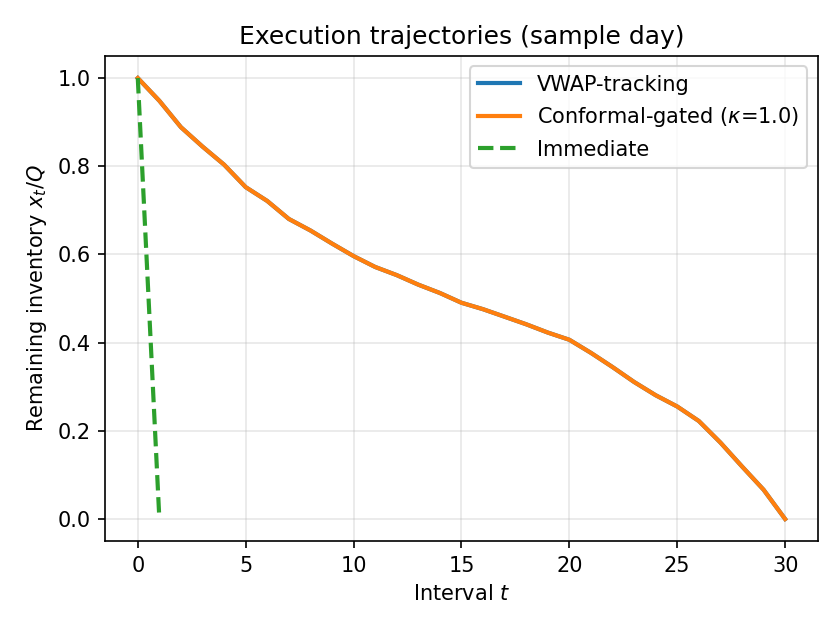
\includegraphics[width=4.375in,keepaspectratio]{./media/image21.png}\end{center}
\caption{Execution trajectories on a sample session: remaining inventory over time for VWAP-tracking, Conformal-gated, and Immediate.}
\label{fig:9}
\end{figure}

\begin{figure}[htbp]
\centering
\begin{center}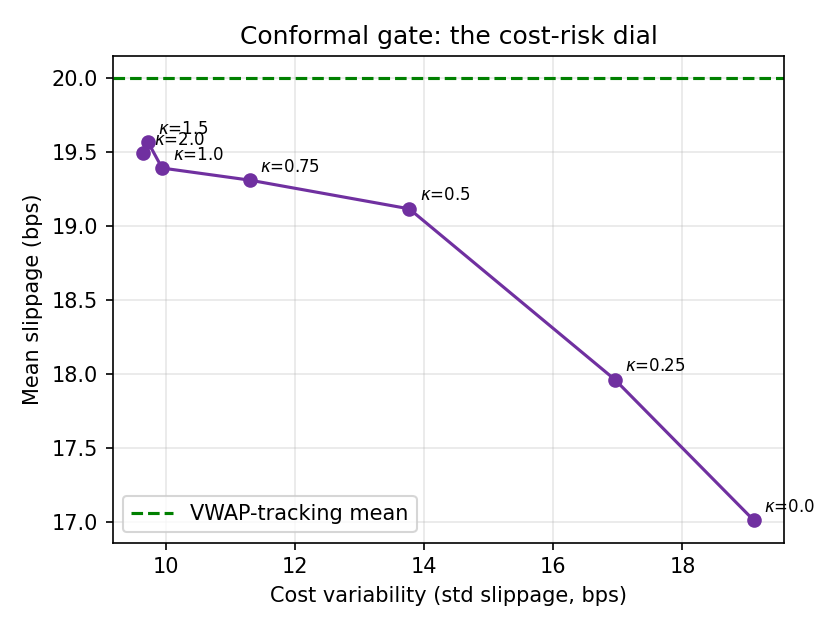
\includegraphics[width=4.375in,keepaspectratio]{./media/image22.png}\end{center}
\caption{The conformal gate as a cost--risk dial. Sweeping the gate threshold traces a frontier from aggressive forecast-following to conservative tracking; dashed line marks the VWAP-tracking mean.}
\label{fig:10}
\end{figure}

The PPO agent is a cautionary case. Pooled over three training seeds, it
attains 33.9 bps mean slippage with a large standard deviation of 115.9
bps: worse on both axes than the strong volume-aware schedules
(VWAP-tracking and TWAP), though it does improve on the front-loading
Almgren--Chriss schedule. Individual runs ranged from competitive with
VWAP-tracking to substantially worse, so any single-seed report would
give a misleading impression. It is this instability, rather than a
tuning artefact, that is the salient result.

\section{Real-Data Validation}

To test whether the simulator findings transfer, we re-ran the conformal
pipeline on real intraday data: thirty large-capitalisation US equities,
5-minute bars over sixty trading days (about 1,800 ticker-days),
bucketed into T = 13 intervals. The split into training, calibration,
and test sessions is strictly time-ordered, 50/25/25, leaving 450
held-out test sessions, so that calibration never sees the future and
there is no look-ahead. The intraday volume curve is now empirical
rather than a synthetic U-shape. The market-impact model is left
unchanged (linear in participation with fixed η), since it cannot be
estimated from bar data; absolute slippage levels are therefore
model-dependent, and only relative comparisons across policies should be
read as meaningful.

The central result is that the predictor's coverage transfers to real
markets. At the 90\% nominal level, empirical coverage on the held-out
real sessions is 90.7\%, and the reliability curve (Figure 11) tracks
the diagonal across the full range of nominal levels. Since real
intraday returns are non-exchangeable, this validity is not guaranteed a
priori, and its empirical confirmation is the key real-data finding. It
also answers the concern that coverage in the synthetic study held only
because exchangeability was true by construction.

\begin{figure}[htbp]
\centering
\begin{center}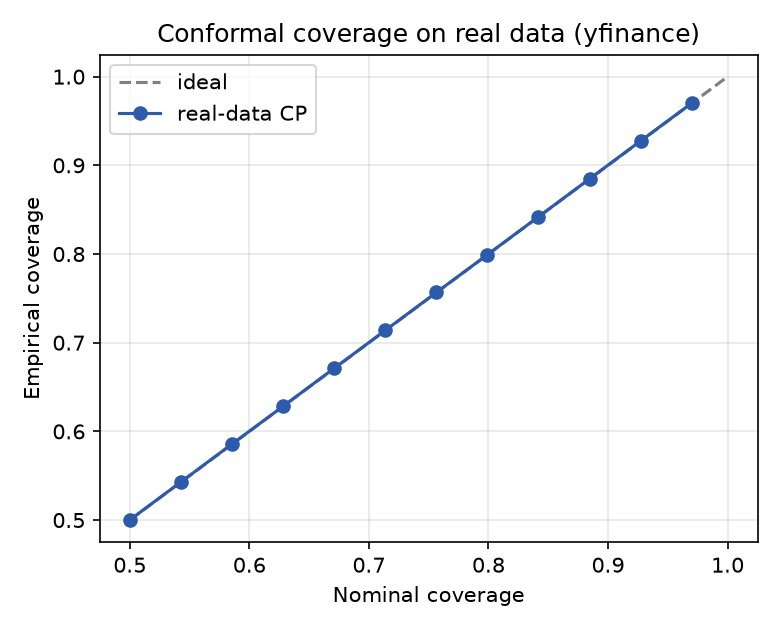
\includegraphics[width=3.750in,keepaspectratio]{./media/image23.png}\end{center}
\caption{Conformal coverage on real intraday data (30 US large-caps, 5-minute bars, 450 held-out sessions). Empirical coverage tracks the nominal level closely across the range, including 90.7\% at the 90\% operating point.}
\label{fig:11}
\end{figure}

Execution performance on the real test sessions is reported in Table 2
and Figure 12. The variance-reduction mechanism survives: gating lowers
the standard deviation of slippage from 2.60 bps (Forecast-greedy) to
2.06 bps at κ = 1.0, a 21\% reduction, while VWAP-tracking again
provides the zero-variance reference. The forecast edge itself, however,
is small. Real 5-minute returns on liquid large-caps are far less
predictable than the simulator's AR(1) dynamics, so Forecast-greedy
improves mean slippage over VWAP-tracking by only about 0.2 bps, and
gating then trades most of that thin edge for lower variance, converging
toward the benchmark. The real-data frontier is consequently compressed.
The conformal machinery behaves exactly as designed, but at this
frequency and liquidity the timing signal is weak, so the practical
payoff is reproducibility and risk control rather than a large cost
saving.

\textbf{Table 2.} Execution performance on 450 held-out real intraday
sessions (yfinance, 5-minute bars). Lower is better on both axes;
conformal-gated rows highlighted.

\begin{longtable}[]{@{}llll@{}}
\toprule
\begin{minipage}[b]{0.22\columnwidth}\raggedright
\textbf{Method}\strut
\end{minipage} & \begin{minipage}[b]{0.22\columnwidth}\raggedright
\textbf{Slippage vs VWAP}

\textbf{mean (bps)}\strut
\end{minipage} & \begin{minipage}[b]{0.22\columnwidth}\raggedright
\textbf{Slippage vs VWAP}

\textbf{std (bps)}\strut
\end{minipage} & \begin{minipage}[b]{0.22\columnwidth}\raggedright
\textbf{Class}\strut
\end{minipage}\tabularnewline
\midrule
\endhead
TWAP & 24.2 & 14.2 & Schedule\tabularnewline
VWAP-tracking & 20.0 & 0.0 & Schedule\tabularnewline
Forecast-greedy & 19.8 & 2.60 & Forecast\tabularnewline
\rowcolor{gray!18}Conformal-gated ($\kappa$=0.5) & 19.9 & 2.14 & Conformal\tabularnewline
\rowcolor{gray!18}Conformal-gated ($\kappa$=1.0) & 19.9 & 2.06 & Conformal\tabularnewline
\bottomrule
\end{longtable}

\begin{figure}[htbp]
\centering
\begin{center}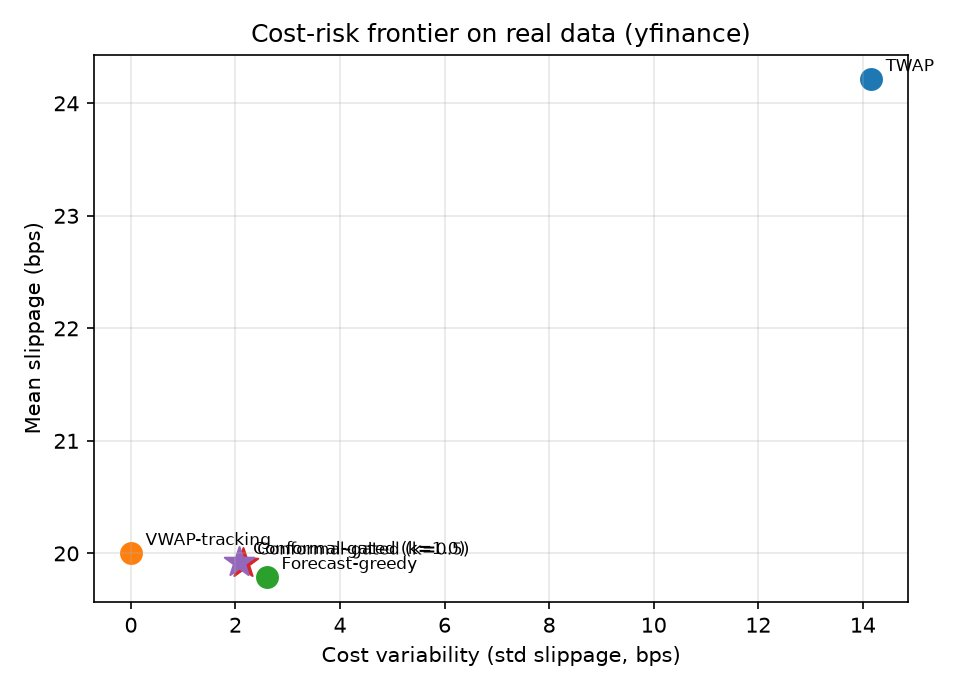
\includegraphics[width=4.583in,keepaspectratio]{./media/image24.png}\end{center}
\caption{Cost--risk frontier on real intraday data. The forecast-based policies cluster near the VWAP-tracking benchmark: gating reduces variance, but the mean edge over VWAP-tracking is small at this frequency and liquidity.}
\label{fig:12}
\end{figure}

We regard this as the more credible outcome. It confirms that the
conformal layer's guarantee is robust to the move from simulation to
real markets, while remaining candid that the size of any tradable edge
is data-dependent and, for these instruments, modest. The natural place
to look for a larger edge, and hence more value from gating, is markets
with stronger short-horizon structure (less liquid names,
higher-volatility regimes, event windows) or higher-frequency
limit-order-book data.

\section{Discussion}

The comparison helps locate where the value of uncertainty
quantification actually lies. A point forecast is double-edged. It can
lower average cost, but it also adds variance, because every forecast is
sometimes wrong and acting on all of them realises those errors. The
conformal interval supplies what is otherwise missing: a calibrated
measure of when the forecast can be trusted. Used as a gate, it lets the
policy harvest the reliable signals and decline the unreliable ones, and
because the gate is an explicit rule with a coverage interpretation, its
behaviour is predictable and its risk dial is directly controllable. The
off-the-shelf RL agent has a harder task. It must discover both the
timing signal and the appropriate degree of caution from a scalar
reward, and in our experiments it does so unreliably across seeds. We do
not read this as evidence that RL cannot succeed here; a tuned,
risk-sensitive agent may well match or exceed the gate. The point is
narrower: for the same problem, a transparent conformal gate reaches a
competitive operating point with far greater reproducibility and at a
fraction of the engineering effort.

\section{Limitations}

\begin{itemize}
\item
  The forecast edge is partly endogenous to the simulator. Short-horizon
  predictability is built into the AR(1) data-generating process, so the
  large edge seen in simulation overstates what is achievable in
  practice. The real-data validation (§6) addresses this directly: on
  real 5-minute equity data the forecast edge over VWAP-tracking shrinks
  to about 0.2 bps, which confirms that the simulator inflates magnitude
  even though the mechanism itself transfers.
\end{itemize}

\begin{itemize}
\item
  Conformal coverage transferred well to the real intraday data we
  tested (90.7\% at the 90\% level), but only on liquid US large-caps at
  5-minute frequency. Behaviour under regime shifts, in less liquid
  names, or on higher-frequency limit-order-book data is not
  established, and online or adaptive conformal methods (Gibbs \&
  Candès, 2024; Zaffran et al., 2022; Barber et al., 2023) were not
  benchmarked.
\item
  The study is simulator-based. Market impact is an assumed
  linear-participation model rather than one estimated from fills, and
  the price and volume processes omit limit-order-book microstructure
  and cross-asset effects.
\item
  The reinforcement-learning agent is a single off-the-shelf PPO
  configuration trained on a modest budget, so its underperformance
  reflects this particular setup rather than a general claim about RL.
  Stronger algorithms, larger budgets, and explicit risk-sensitive or
  distributional objectives could change the learned-agent picture; a
  fully tuned RL baseline is left to future work.
\item
  No live-trading efficacy is claimed. Results are out-of-sample only
  with respect to simulated seeds, and latency and partial fills are not
  modelled.
\end{itemize}

\section{Conclusion}

We have presented a reproducible study of VWAP-benchmarked execution,
comparing classical schedules, a reinforcement-learning agent, and
conformal forecast-driven policies within a single MDP. In simulation, a
normalised split-conformal predictor delivered valid coverage, and
gating forecast-driven trades by the conformal interval produced a
tunable, reproducible reduction in execution-cost variance, reaching a
better cost--risk operating point than an off-the-shelf PPO agent.
Validation on real intraday data then confirmed that the coverage
guarantee transfers (90.7\% empirical at the 90\% level) and that the
variance-reduction mechanism persists, while showing honestly that the
forecast edge on liquid large-caps at 5-minute frequency is small. The
conformal gate is therefore best understood as a dependable and
transparent component for uncertainty-aware execution, one whose
statistical validity holds on real data even where the tradable edge is
modest. Several directions follow naturally: higher-frequency
limit-order-book data and less liquid instruments, where short-horizon
structure is stronger; adaptive conformal calibration under regime
change; a tuned, risk-sensitive RL baseline; and the combination of
conformal gating with a learned base policy.

\section*{Author Contributions}

A. Irshad: conceptualisation (supporting), software, validation, formal
analysis, investigation, data curation, visualisation, writing original
draft. S. Biswas: conceptualisation (lead), methodology, supervision,
formal analysis (supporting), writing review and editing. Both authors
read and approved the final manuscript. (Roles follow the CRediT
taxonomy.)

\section*{Data and Code Availability}

The simulated experiments (§§3--5) use no proprietary data and are
generated entirely by the synthetic simulator described in Section 3.
The real-data validation (Section 6) uses publicly available intraday
price and volume data for thirty US large-cap equities (5-minute bars),
retrieved through the Yahoo Finance API; no licensed or proprietary
datasets are used. The complete source code --- the market simulator,
conformal predictor, baselines, reinforcement-learning agent, the
real-data validation pipeline, and the scripts that reproduce every
table and figure --- is released to enable full reproduction. Fixed
random seeds are used throughout and reported in the code, and the
real-data validation can be re-run directly against the public data
source.

\section*{Conflict of Interest}

The authors declare no competing financial or non-financial interests
relevant to this work. No external funding was received.

\section*{References}
\begingroup
\small
\setlength{\parindent}{0pt}
\setlength{\parskip}{5pt}
\everypar{\hangindent=1.5em}
Almgren, R., \& Chriss, N. (2001). Optimal execution of portfolio
transactions. Journal of Risk, 3(2), 5--40.

Angelopoulos, A. N., \& Bates, S. (2023). Conformal prediction: A gentle
introduction. Foundations and Trends in Machine Learning, 16(4),
494--591.

Barber, R. F., Candès, E. J., Ramdas, A., \& Tibshirani, R. J. (2023).
Conformal prediction beyond exchangeability. Annals of Statistics,
51(2), 816--845.

Bertsimas, D., \& Lo, A. W. (1998). Optimal control of execution costs.
Journal of Financial Markets, 1(1), 1--50.

Cartea, Á., Jaimungal, S., \& Penalva, J. (2015). Algorithmic and
High-Frequency Trading. Cambridge University Press.

Cartea, Á., Jaimungal, S., \& Sánchez-Betancourt, L. (2023).
Reinforcement learning for algorithmic trading. In Machine Learning and
Data Sciences for Financial Markets. Cambridge University Press.

Gatheral, J. (2010). No-dynamic-arbitrage and market impact.
Quantitative Finance, 10(7), 749--759.

Gibbs, I., \& Candès, E. J. (2024). Conformal inference for online
prediction with arbitrary distribution shifts. Journal of Machine
Learning Research, 25(162), 1--36.

Hambly, B., Xu, R., \& Yang, H. (2023). Recent advances in reinforcement
learning in finance. Mathematical Finance, 33(3), 437--503.

Lei, J., G'Sell, M., Rinaldo, A., Tibshirani, R. J., \& Wasserman, L.
(2018). Distribution-free predictive inference for regression. Journal
of the American Statistical Association, 113(523), 1094--1111.

Lin, S., \& Beling, P. A. (2020). An end-to-end optimal trade execution
framework based on proximal policy optimization. Proceedings of the 29th
International Joint Conference on Artificial Intelligence (IJCAI),
4548--4554.

Macrì, A., \& Lillo, F. (2024). Reinforcement learning for optimal
execution when liquidity is time-varying. Applied Mathematical Finance,
31(5), 312--342.

Nagy, P., Calliess, J., \& Zohren, S. (2023). Asynchronous deep double
dueling Q-learning for trading-signal execution in limit order book
markets. Frontiers in Artificial Intelligence, 6, 1151003.

Nevmyvaka, Y., Feng, Y., \& Kearns, M. (2006). Reinforcement learning
for optimized trade execution. Proceedings of the 23rd International
Conference on Machine Learning (ICML), 673--680.

Ning, B., Lin, F. H. T., \& Jaimungal, S. (2021). Double deep Q-learning
for optimal execution. Applied Mathematical Finance, 28(4), 361--380.

Obizhaeva, A. A., \& Wang, J. (2013). Optimal trading strategy and
supply/demand dynamics. Journal of Financial Markets, 16(1), 1--32.

Perold, A. F. (1988). The implementation shortfall: Paper versus
reality. Journal of Portfolio Management, 14(3), 4--9.

Romano, Y., Patterson, E., \& Candès, E. (2019). Conformalized quantile
regression. Advances in Neural Information Processing Systems, 32,
3543--3553.

Schulman, J., Wolski, F., Dhariwal, P., Radford, A., \& Klimov, O.
(2017). Proximal policy optimization algorithms. arXiv:1707.06347.

Stankevičiūtė, K., Alaa, A. M., \& van der Schaar, M. (2021). Conformal
time-series forecasting. Advances in Neural Information Processing
Systems, 34, 6216--6228.

Sun, S., Wang, R., \& An, B. (2023). Reinforcement learning for
quantitative trading. ACM Transactions on Intelligent Systems and
Technology, 14(3), 1--29.

Sutton, R. S., \& Barto, A. G. (2018). Reinforcement Learning: An
Introduction (2nd ed.). MIT Press.

Tibshirani, R. J., Foygel Barber, R., Candès, E., \& Ramdas, A. (2019).
Conformal prediction under covariate shift. Advances in Neural
Information Processing Systems, 32, 2530--2540.

Vovk, V., Gammerman, A., \& Shafer, G. (2005). Algorithmic Learning in a
Random World. Springer.

Xu, C., \& Xie, Y. (2023). Sequential predictive conformal inference for
time series. Proceedings of the 40th International Conference on Machine
Learning (ICML), 38707--38727.

Zaffran, M., Féron, O., Goude, Y., Josse, J., \& Dieuleveut, A. (2022).
Adaptive conformal predictions for time series. Proceedings of the 39th
International Conference on Machine Learning (ICML), 25834--25866.
\endgroup


\end{document}
